\chapter[Referencial Teórico]{Referencial Teórico}
Neste capítulo são apresentadas as bases teóricas para o desenvolvimento do \textit{framework}. O capítulo está organizado em seções. Na seção 2.1 faz-se referência ao contexto de Verificação e Validação de Software. Na seção 2.2 aborda-se uma temática mais específica da qualidade de software, os testes. Traz a motivação para fazê-los, bem como uma descrição sobre os níveis de testes e as vantagens e estratégias de automatizá-los. Na seção 2.3 dicuti-se sobre \textit{frameworks}, sua definição, motivação, vantagens e desvantagens e classificação. Na seção 2.4 explana-se sobre a geração de testes e técnicas de implementá-la.

\section{Verificação e Validação de Software}
Software é uma atividade que requer um processo com o envolvimento de diversas atividades e diferentes pessoas. Essa característica permite a inserção de defeitos no produto final \cite{trodo_2009}. Além disso, há o risco de produzir-se algo que não foi solicitado, devido ao mal entendimento dos requisitos\textsuperscript{Falta referência}. Esse conjunto de fatores fez surgir maior preocupação em relação a qualidade de software e, inclusive nesse contexto, é que há o advento da Engenharia de Software, com o objetivo de produzir softwares com qualidade \cite{bueno_e_campelo_2013}.
\par
\indent Tendo em vista o cuidado com o nível dos softwares surge a necessidade de conceituar qualidade no que tange esse assunto. Essa definição é díficil, pois qualidade é um conceito abstrato. Em essência, a qualidade esta ligada a possibilidade de medir determinado atributo e comparar o resultado com padrões já conhecidos \cite{bueno_e_campelo_2013}. No âmbito de software há também o conceito de métricas. Elas são utilizadas para dar visibilidade de determinadas características do produto, de forma a demonstrar o tamanho, esforço e complexidade do software em construção, dentre outros atributos \cite{abreu_2011}.
\par
\indent Tendo isso em vista, observa-se que, no que se refere ao software, tem-se como caracterizar a qualidade em dois tipos, na medida em que há características mensuráveis tanto no projeto quanto no produto. São eles: qualidade de projeto e qualidade de conformidade. O primeiro diz respeito aos requisitos, especificações e arquitetura, enquanto que o segundo foca na implementação e sua conformidade com o que foi especificado \cite{bueno_e_campelo_2013}.
\par
\indent A qualidade de software está ligada a atividade de verificação e validação de software \cite{bueno_e_campelo_2013}. A qualidade de software é uma atividade que pertence ao ambiente de gerência, enquanto que a verificação e validação de software é uma prática mais técnica e enquadra-se no desenvolvimento do produto \cite{bueno_e_campelo_2013}. Segundo \citeonline{sommerville_2007}, verificação e validação de software é o processo, que certifica que o produto em desenvolvimento atende as especificações esperadas pelo cliente. Essa atividade deve permear todo o processo de produção do software, de forma a garantir que o produto respeita o especificado desde o início. Essa prática evita que a identificação de defeitos seja percebido apenas ao final do desenvolvimento, o que aumentaria os custos do projeto.
\par
\indent Verificação e validação são dois conceitos muitas vezes confundidos. Verificação de software busca analisar se o produto está em conformidade com o que foi especificado. É nessa atividade que observa-se o quão próximo está o produto das especificações dos requisitos, sejam eles funcionais ou não funcionais \cite{sommerville_2007}. A validação de software objetiva garantir que o software é o que o cliente solicitou \cite{sommerville_2007}. Assim, pode-se conceituar verificação e validação da seguinte forma:
\begin{itemize}
\item Verificação: análise sobre o produto, afim de observar se o produto está sendo feito de maneira certa.
\item Validação: avalia se o produto em construção é o correto em relação às expectativas do cliente.
\end{itemize}
\par
\indent O processo de verificação e validação é responsável por gerar a certeza de que o software está adequado ao que foi pedido \cite{sommerville_2007}. Para essa tarefa a verificação e validação utiliza-se de duas abordagens: inspeções de software e testes de software. Inspeção de software é um processo estático, o que significa que não há a necessidade do sistema está em funcionamento. Essa atividade é baseada em revisões, com o intuito de identificar erros e omissões. Toda forma de representação do software é passível de uma inspeção (especificações de requisitos, arquitetura etc), no entanto, o código-fonte é um foco \cite{sommerville_2007}. Teste de software é um processo dinâmico, o que exige o funcionamento do software enquanto ele ocorre. Objetiva a demonstração de que o software esta conforme os requisitos, a revelação de falhas ou defeitos no software \cite{sommerville_2007} e a prevenção de novas inserções de defeitos \cite{burke_coyner_2003}.

\section{Testes de Software}
Testes de software é uma atividade que compõe o processo de verificação e validação de software. É uma das técnicas mais utilizadas no âmbito de garantia de confiabilidade de software. Em linhas gerais, é um trabalho de abordagem dinâmica sobre o código-fonte. Isso significa que há a exigência do funcionamento do software para que possa ser realizada essa atividade \cite{barbosa_et_al_2009}. Essa análise dinâmica abre a possiblidade de identificação de defeitos no código-fonte, bem como a prevenção de inserções de novos defeitos. A produção de testes de software fornece, ainda, impulso para atividades de refatoração, manutenção e medição do software \cite{barbosa_et_al_2009}.
\par
\indent Os testes podem ser classificados como: testes caixa-preta e testes caixa-branca \cite{barbosa_et_al_2009}.

\subsection{Testes Caixa-preta}
Testes caixa-preta, também conhecidos como testes baseados em especificações, visam a avaliação do produto em relação aos requisitos funcionais e não funcionais. É caracterizado por fazer análises a partir de documentação e do software em funcionamento, sem necessidade de averiguação do código-fonte \cite{barbosa_et_al_2009}.

\begin{figure}[h]
  \centering
    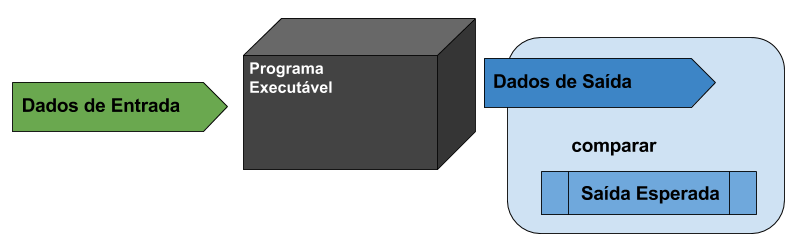
\includegraphics[width=0.8\textwidth]{figuras/test_black_box.png}
    \caption{Diagrama Representativo de Testes Caixa Preta}
    \label{test_black_box}
\end{figure}

A Figura \ref{test_black_box} representa um esquemático do funcionamento de um teste caixa-preta: utiliza-se dados de entrada no software e observa-se a correspondência, ou não, com as expectativas.
\par
\indent Ao utilizar-se de testes caixa-preta desenvolve-se os testes do ponto de vista do usuário, o que auxilia a observar alguma falha nas especificações. Além disso, permite que os casos de teste possam ser produzidos assim que as especificações estiverem prontas \cite{stf_2010}. Essa abordagem de testes também possui pontos negativos, como a pequena quantidade de entradas que podem ser inseridas para testar o produto. Sem especificações claras produzir bons casos de testes caixa-preta torna-se uma tarefa difícil \cite{stf_2010}.

\subsubsection{Técnicas de Derivação de Casos de Teste Caixa-preta}
Testes caixa-preta não são o foco deste trabalho. Dessa forma, apenas um \textit{overview} das técnicas para essa abordagem de testes será abordado. Para a concepção de casos de testes caixa-preta há algumas técnicas utilizadas como guias. São elas: \textbf{particionamento de equivalência}, \textbf{análise de valores limite} e \textbf{gráfico de causa e efeito}.

\begin{description}
\item[Particionamento de Equivalência:] visa a identificação de agrupamentos de casos de testes que cubram diferentes classes de erros. Essa estratégia permite a redução do número de testes que serão produzidos, diminuindo os custos. O particionamento de equivalência divide as entradas do domínio do software em classes. Essas classes devem ser derivadas a partir de um valor significativo para o domínio \cite{williams_2006}.
\end{description}


\subsection{Testes Caixa-branca}
Testes de caixa-branca, também referenciados como testes baseados em programa, almejam a avaliação do produto por meio da execução do código-fonte. Isso possibilita o exercício do software em busca de defeitos para serem corrigidos. Para que ocorra a dinâmica de testes de caixa-branca seleciona-se casos de testes que englobem cenários significativos \cite{barbosa_et_al_2009}.
%%% Técnicas de Derivação de Casos de Teste

%% Níveis de Teste
%%% Testes de Aceitação
%%% Testes de Sistema
%%% Testes de Integração
%%% Testes Unitários
%% Automatização
% Framework
% Geração de Testes
% Resumo do Capítulo